\setbeamercolor{background canvas}{bg=fitblue}
\begin{frame}
\frametitle{Stíny}
\begin{center}
\Huge {\color{white}Stíny}
\end{center}
\end{frame}
\setbeamercolor{background canvas}{bg=white}

\begin{frame}
  \frametitle{Proč potřebujeme stíny?}
  \begin{figure}[h]
    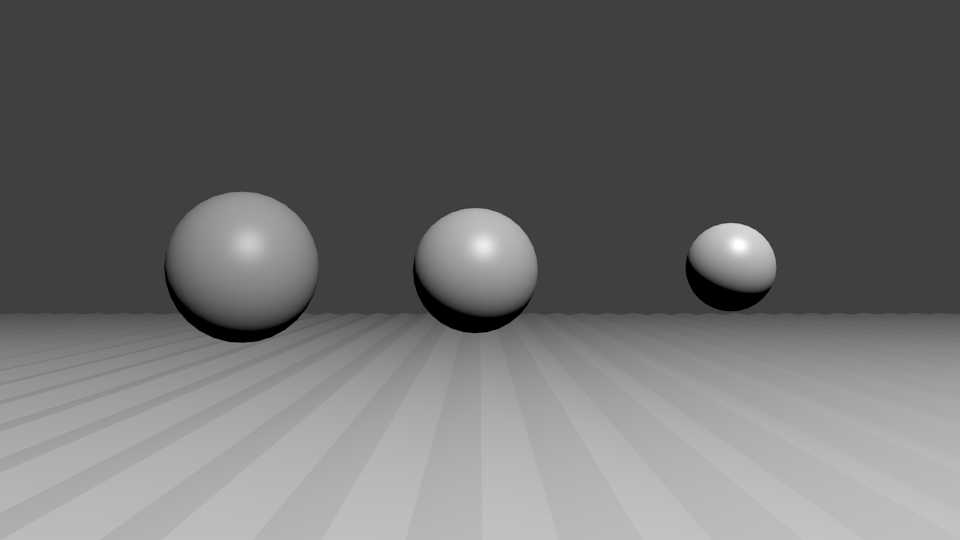
\includegraphics[width=11.5cm,keepaspectratio]{pics/shadows/whyShadows/noShadows}
  \end{figure}
\end{frame}

\begin{frame}
  \frametitle{Proč potřebujeme stíny?}
  \begin{figure}[h]
    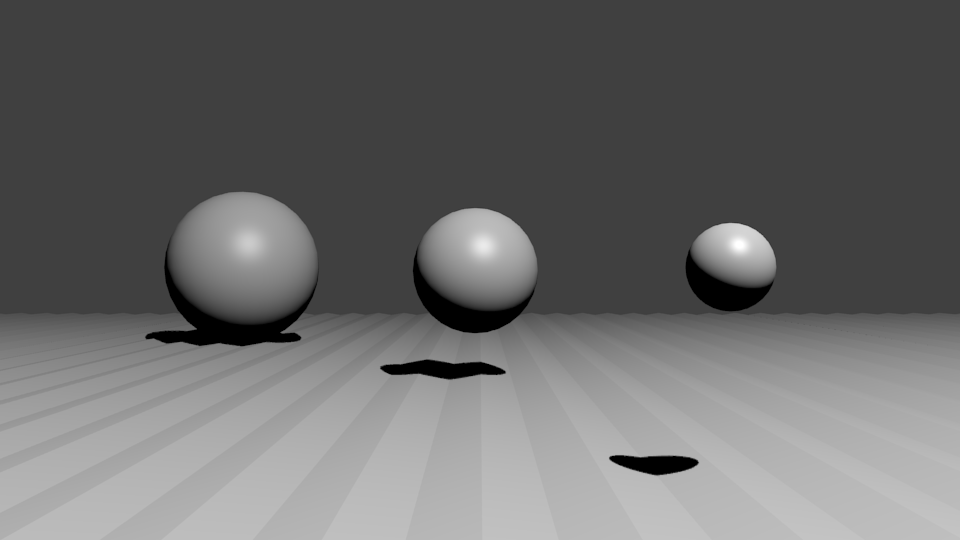
\includegraphics[width=11.5cm,keepaspectratio]{pics/shadows/whyShadows/shadows}
  \end{figure}
\end{frame}

\begin{frame}
  \frametitle{Proč potřebujeme stíny?}
  \begin{figure}[h]
    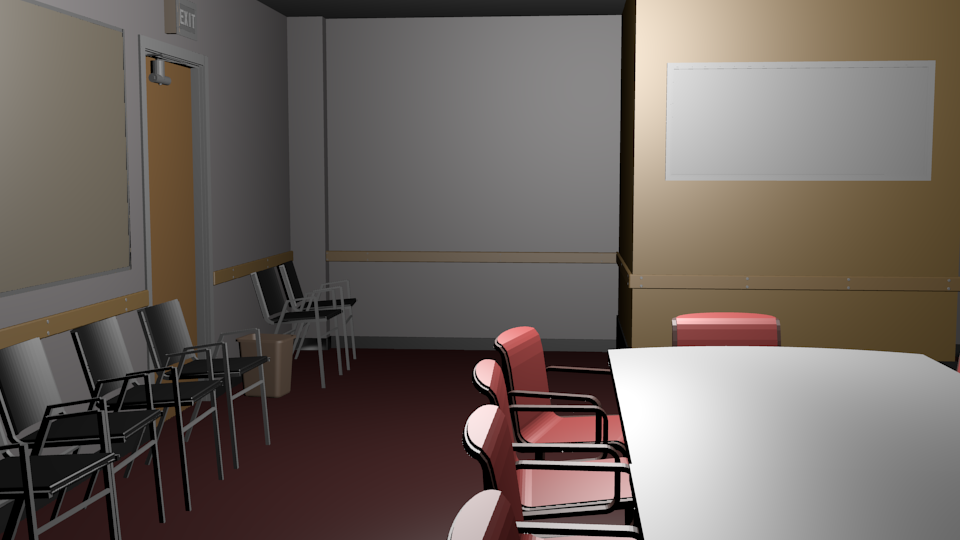
\includegraphics[width=11.5cm,keepaspectratio]{pics/shadows/whyShadows/conferenceNoShadows}
  \end{figure}
\end{frame}

\begin{frame}
  \frametitle{Proč potřebujeme stíny?}
  \begin{itemize}
    \item Stíny pomáhají pochopit 3D scénu.
    \item Vzájemné polohy mezi objekty.
  \end{itemize}
  \begin{figure}[h]
    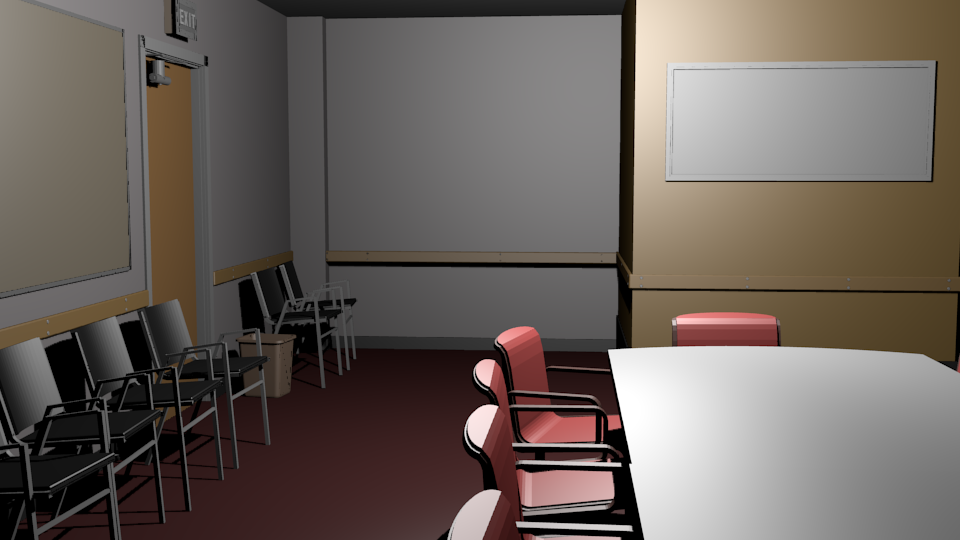
\includegraphics[width=11.5cm,keepaspectratio]{pics/shadows/whyShadows/conferenceShadows}
  \end{figure}
\end{frame}

\begin{frame}
  \frametitle{Druhy světel}
  \begin{itemize}
    \item Omnidirectional point light source.
    \item Spot light source.
    \item Directional light source.
  \end{itemize}
  \begin{figure}[h]
    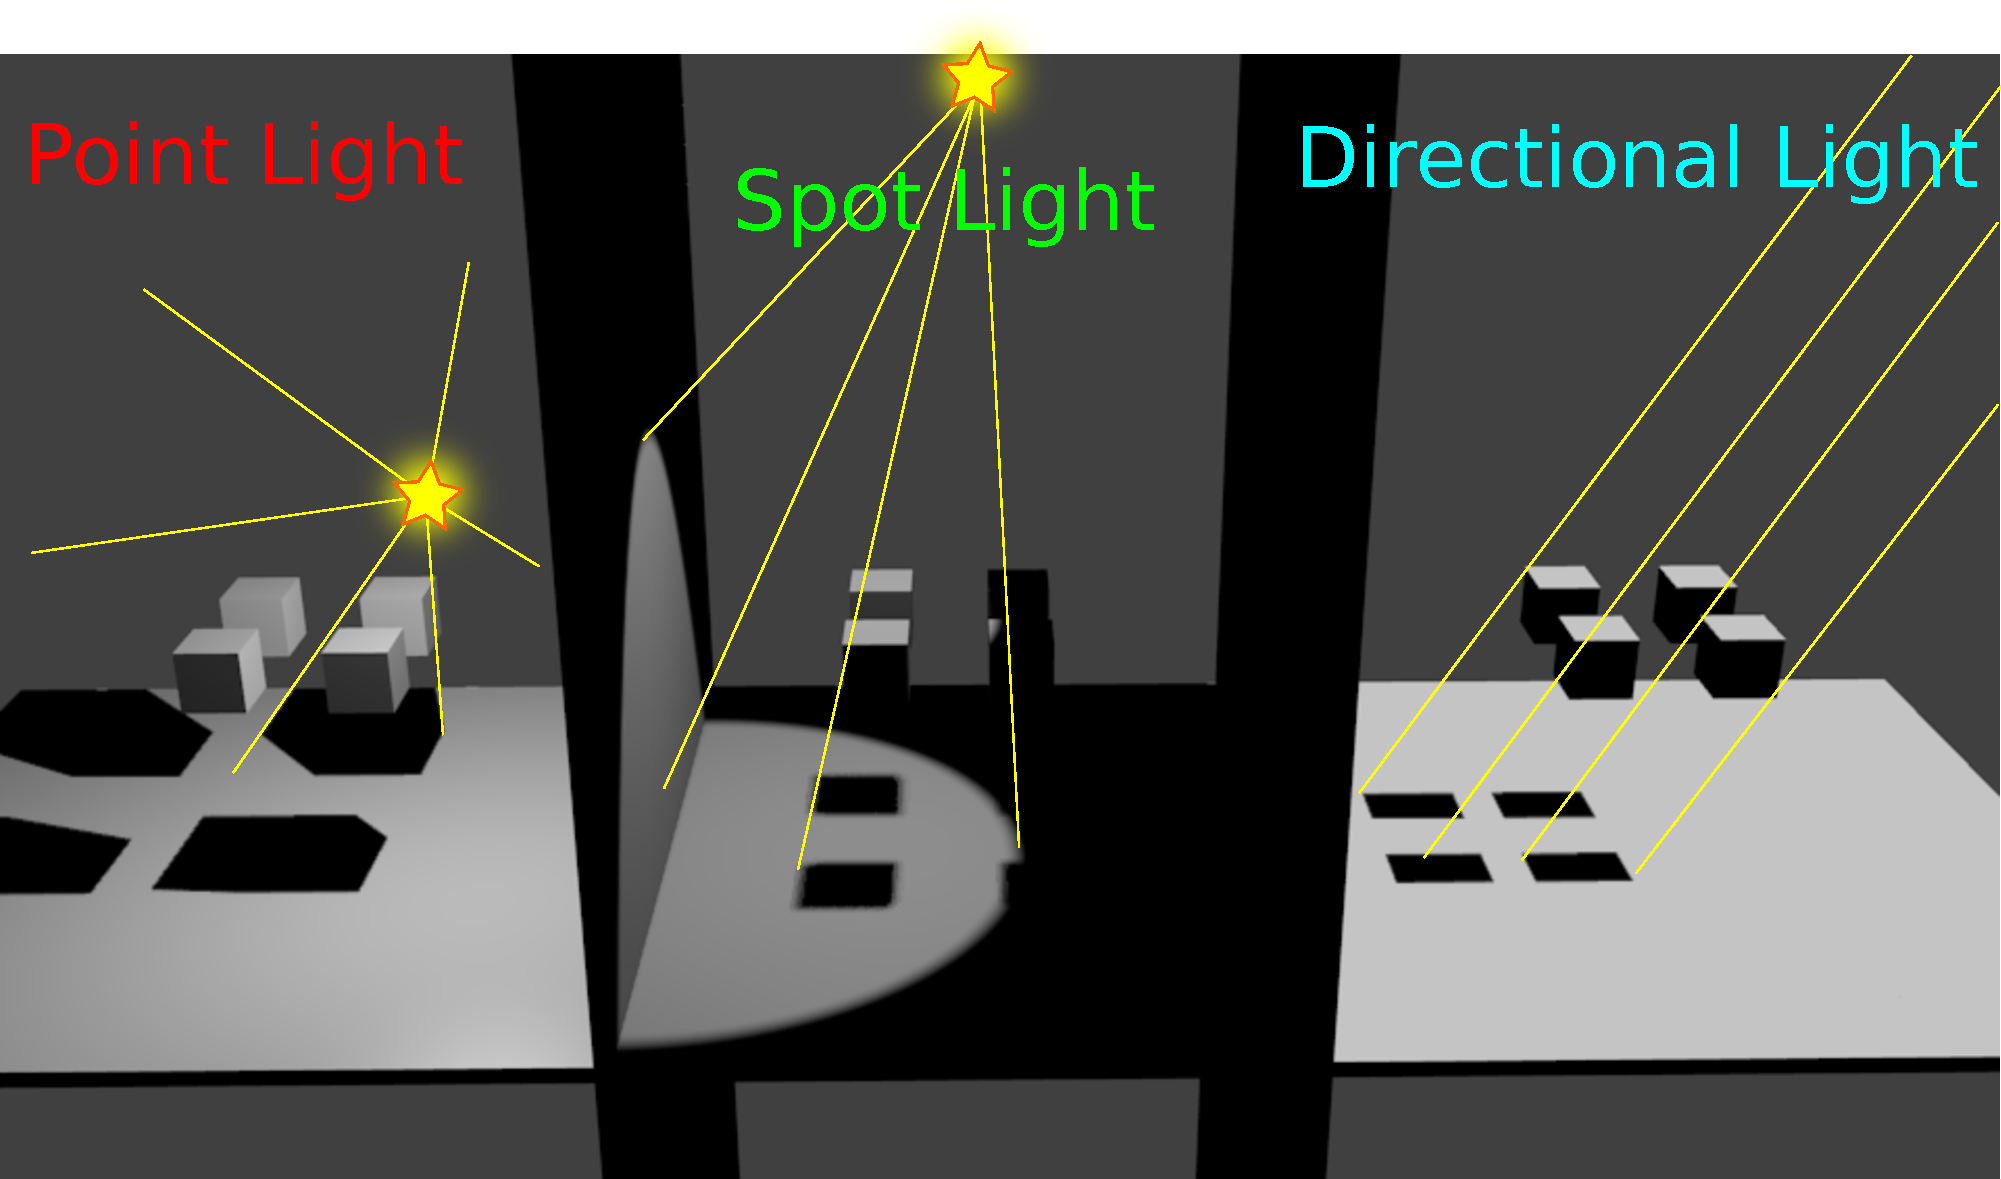
\includegraphics[width=10.5cm,keepaspectratio]{pics/shadows/lightTypes/lightTypes.pdf}
  \end{figure}
\end{frame}

\begin{frame}
  \frametitle{Druhy stínů}
  \begin{itemize}
    \item Tvrdé stíný vznikají z nekonečně malých světelných zdrojů (časté v počítačové grafice).
    \item Měkké stíny vznikají z plošných zdrojů světla.
  \end{itemize}
  \begin{figure}[h]
    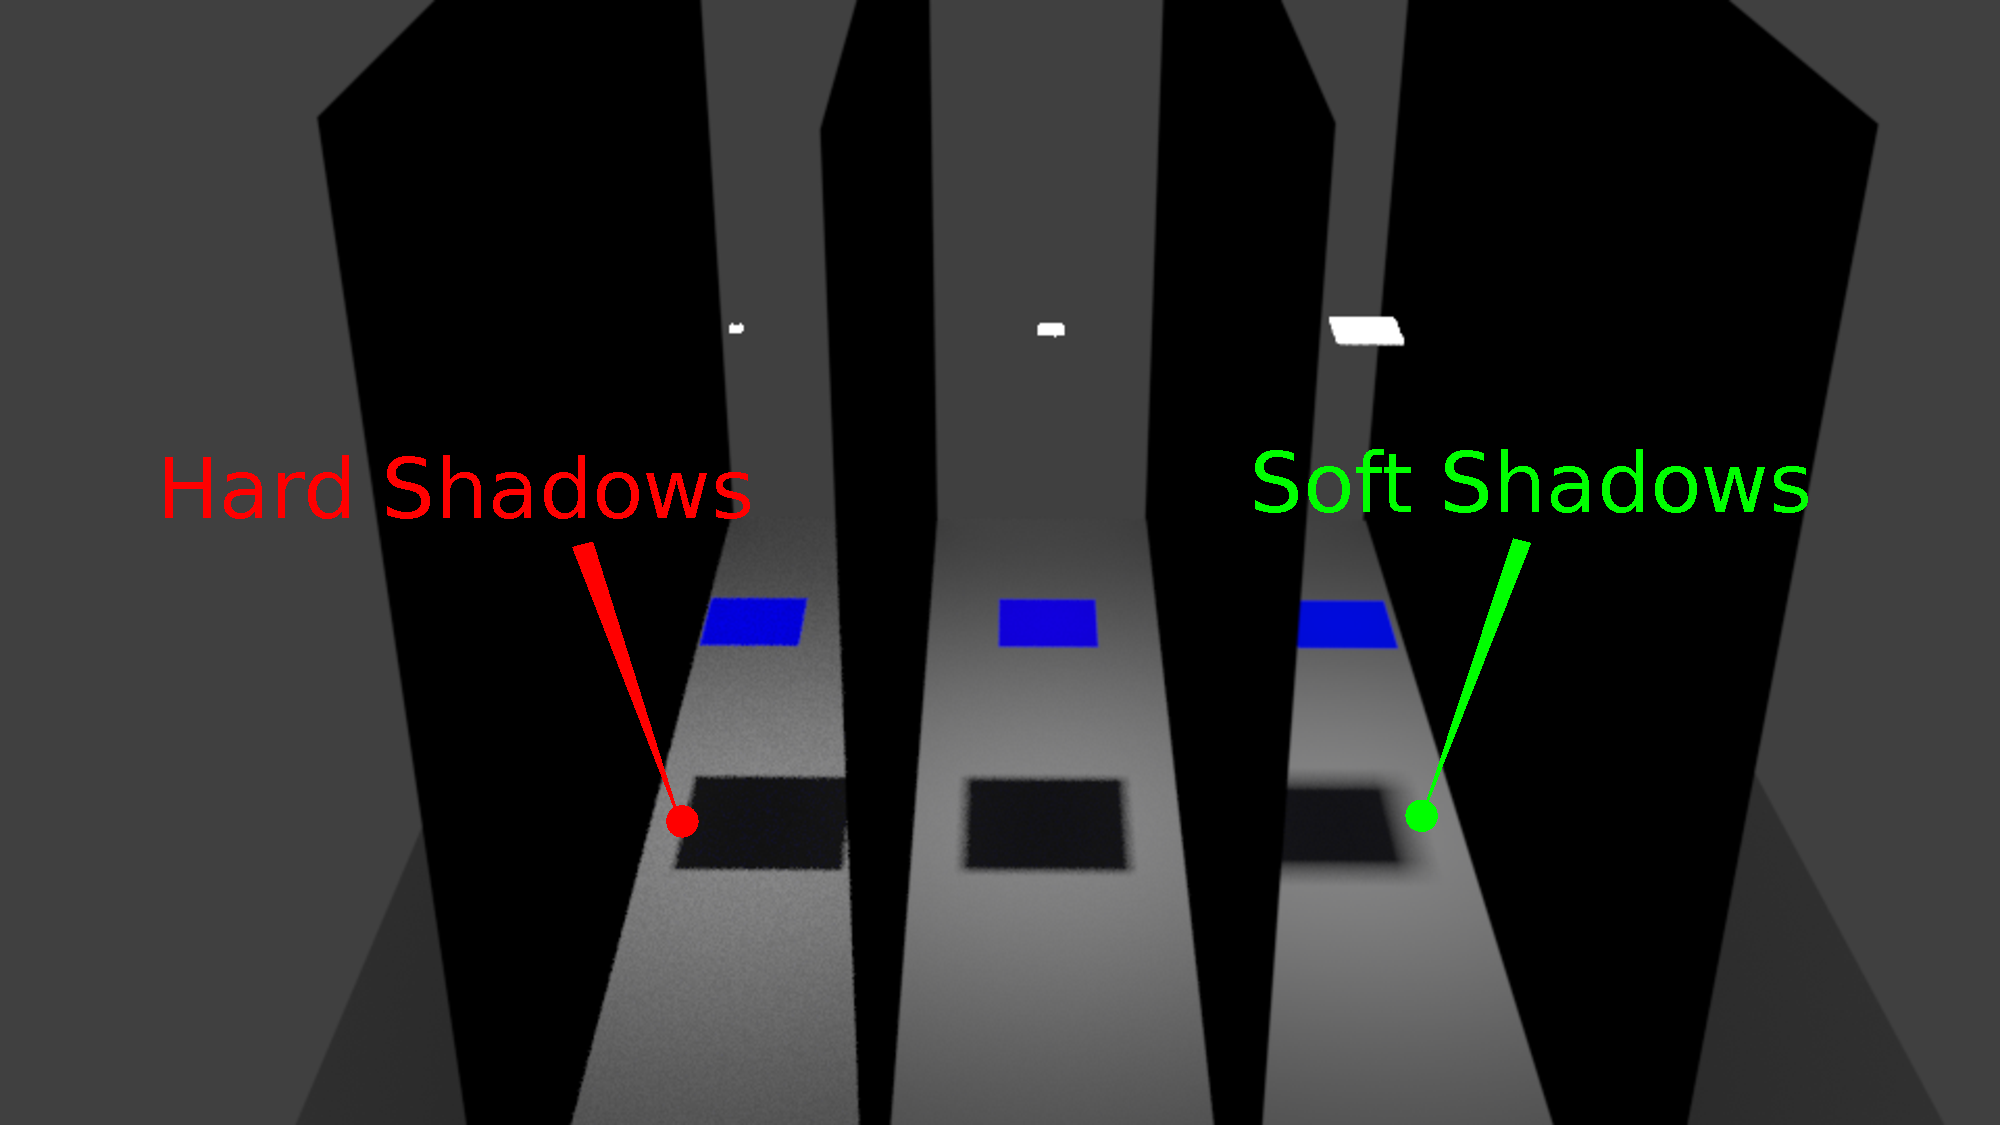
\includegraphics[width=11cm,keepaspectratio]{pics/shadows/hardShadow/hardShadow.pdf}
  \end{figure}
\end{frame}

\begin{frame}
  \frametitle{Druhy stínů}
  \begin{itemize}
    \item Plně osvětlené regiony scény vidí na všechny plošky světla.
    \item Plně zastíněné regiony (umbra) nevidí na žádnou plošku světla.
    \item Polostín (penumbra) vzniká v regionech scény, které vidí jen na některé plošky švětla.
  \end{itemize}
  \begin{figure}[h]
    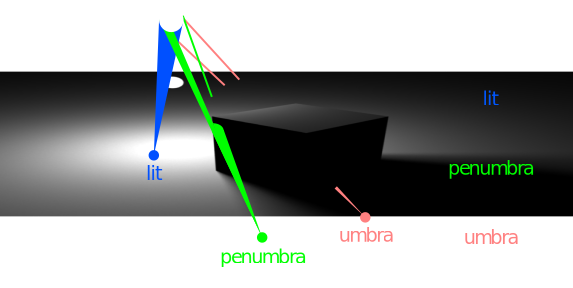
\includegraphics[width=11cm,keepaspectratio]{pics/shadows/penumbra/penumbra}
  \end{figure}
\end{frame}

\begin{frame}
  \frametitle{Druhy stínů}
  \begin{itemize}
    \item Stíny vznikají z přímého osvětlení (můžou být tvrdé, pokud je světlo malé).
    \item Stíny vznikají z nepřímého osvětlení (měkké stíny).
  \end{itemize}
  \begin{figure}[h]
    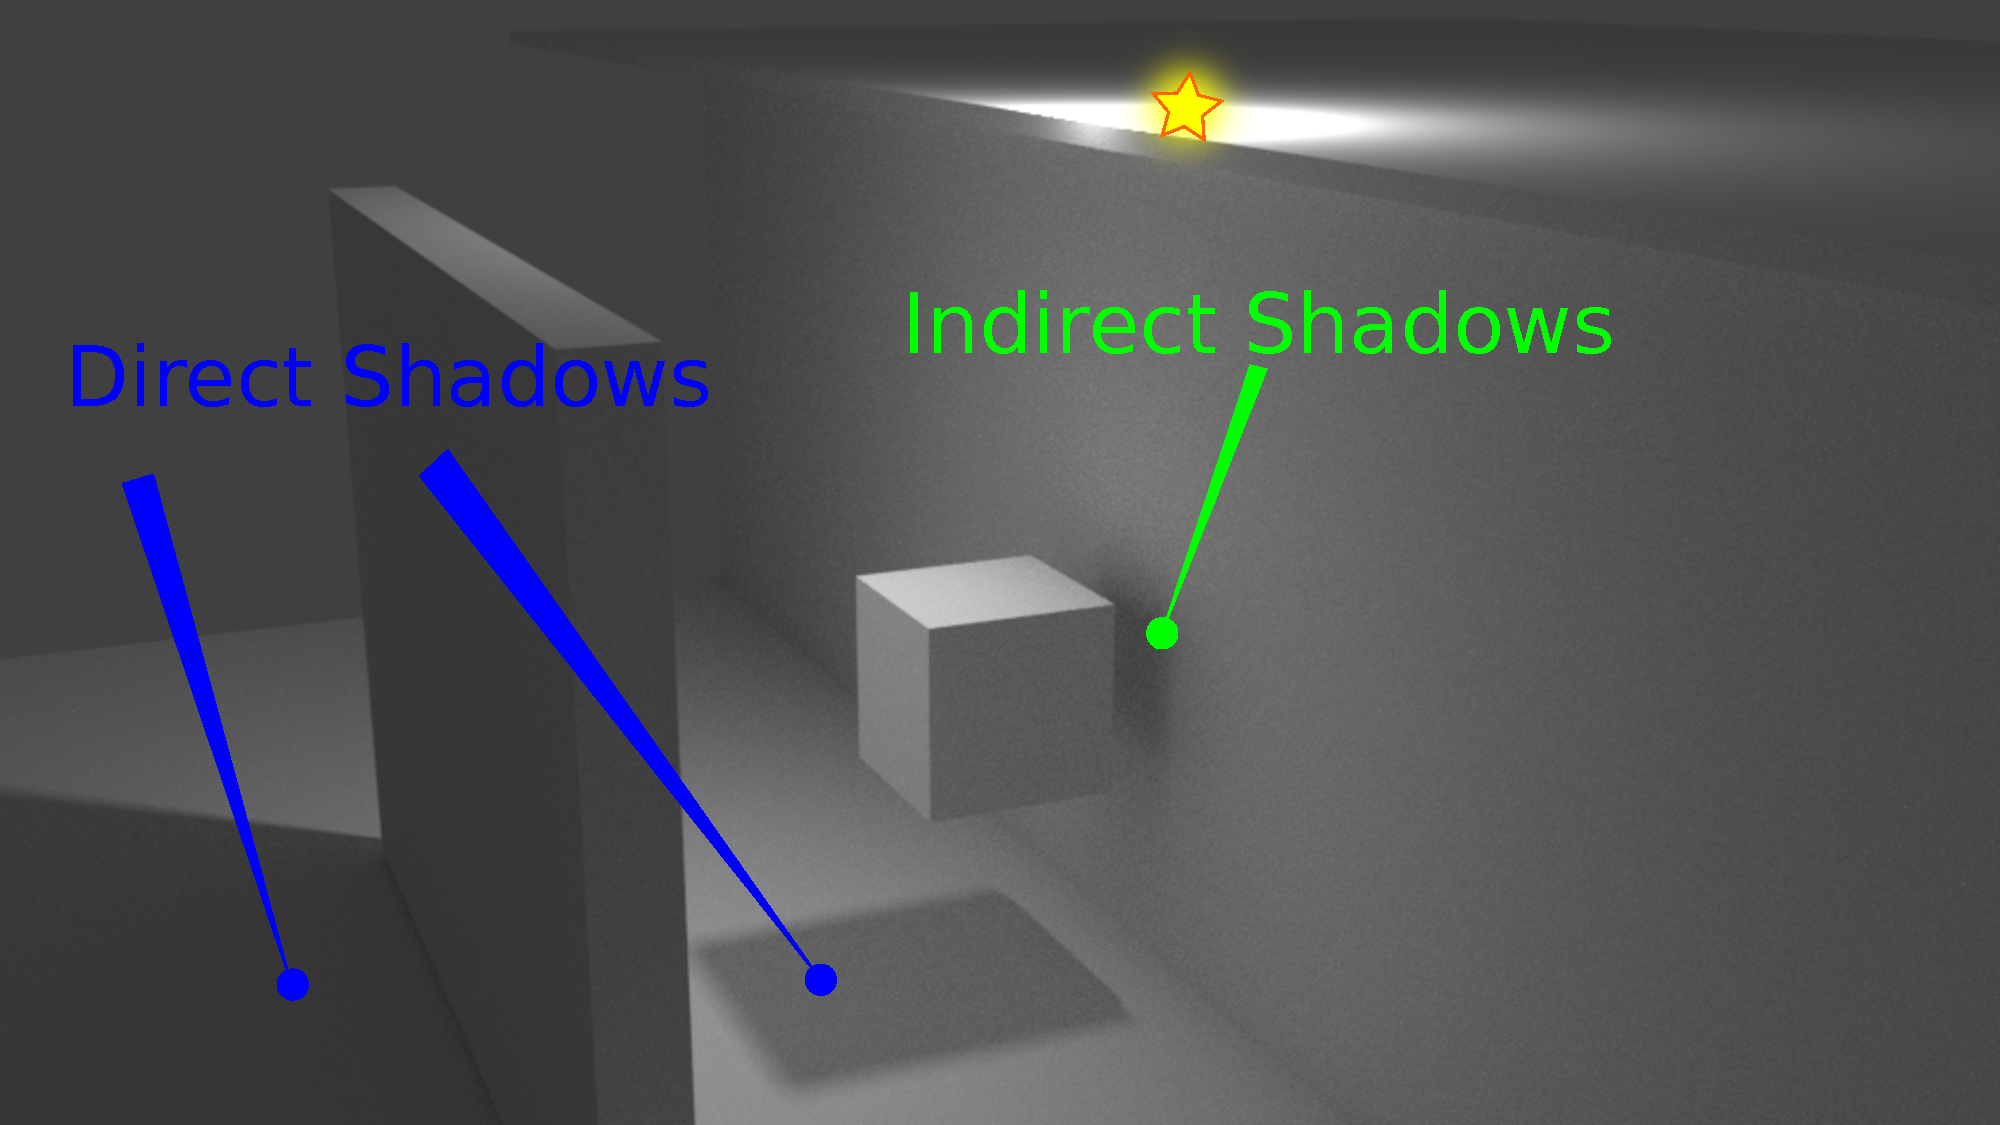
\includegraphics[width=11cm,keepaspectratio]{pics/shadows/indirectShadow/indirectShadows.pdf}
  \end{figure}
\end{frame}

\begin{frame}
  \frametitle{Druhy stínů - Ambient occlusion}
  \begin{itemize}
    \item Ambient occlusion - metoda pro aproximaci části globálního osvětlení a simulaci stínů nepřímého osvětlení.
  \end{itemize}
  \begin{figure}[h]
    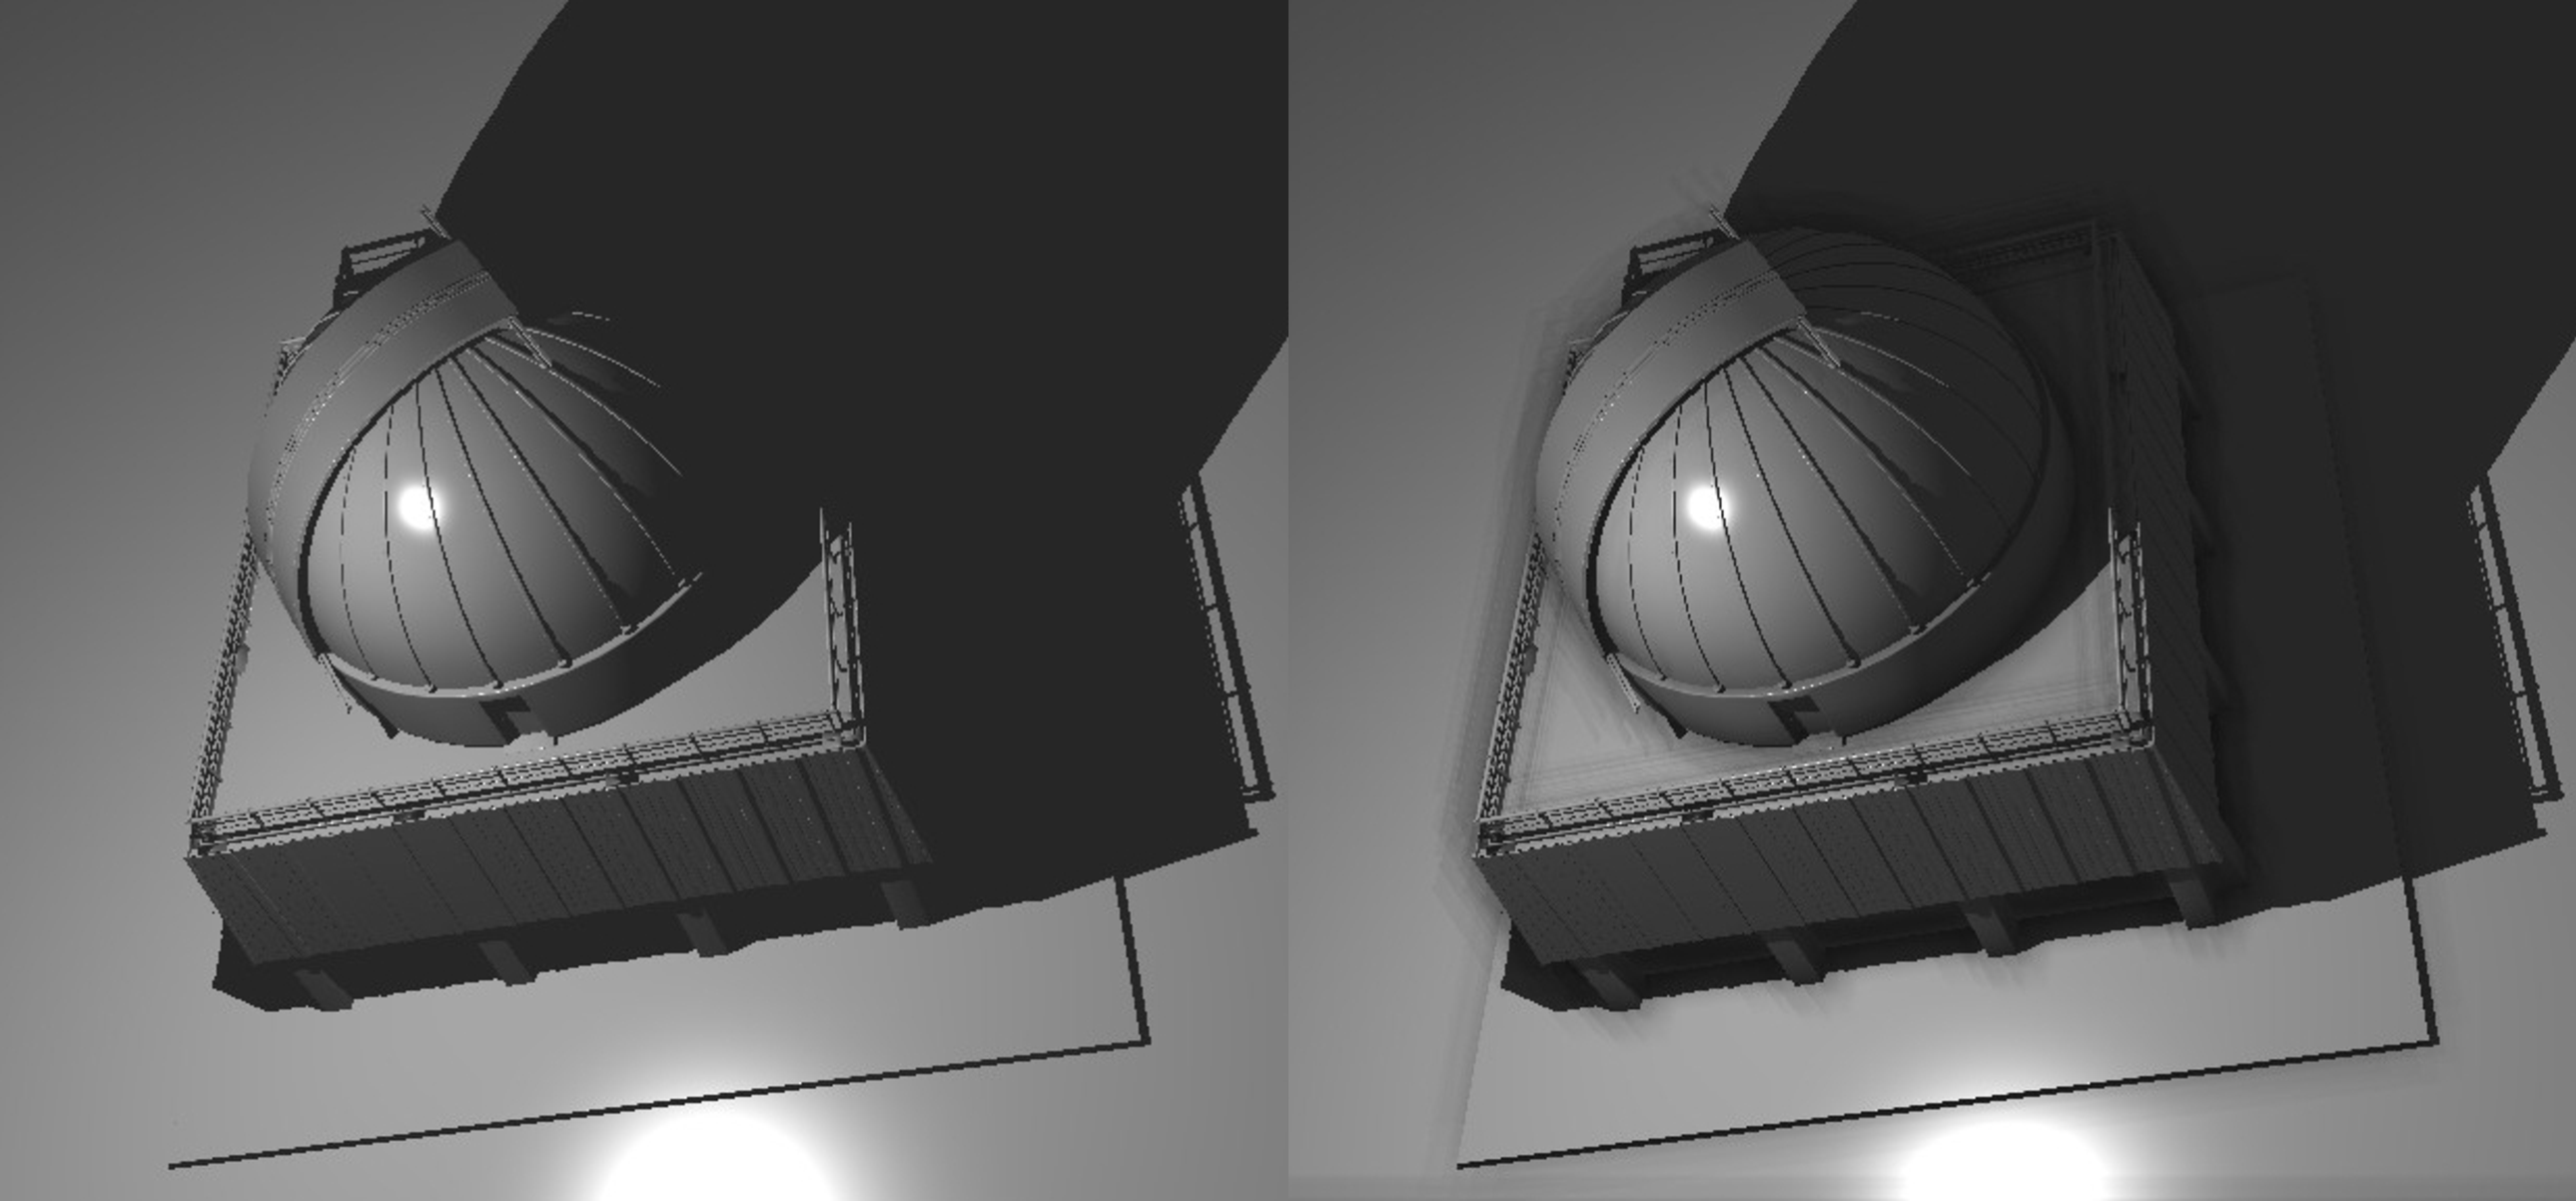
\includegraphics[width=11.5cm,keepaspectratio]{pics/shadows/ambientOcclusion/difference}
  \end{figure}
\end{frame}

\begin{frame}
  \frametitle{Druhy stínů - Ambient occlusion}
  \begin{figure}[h]
    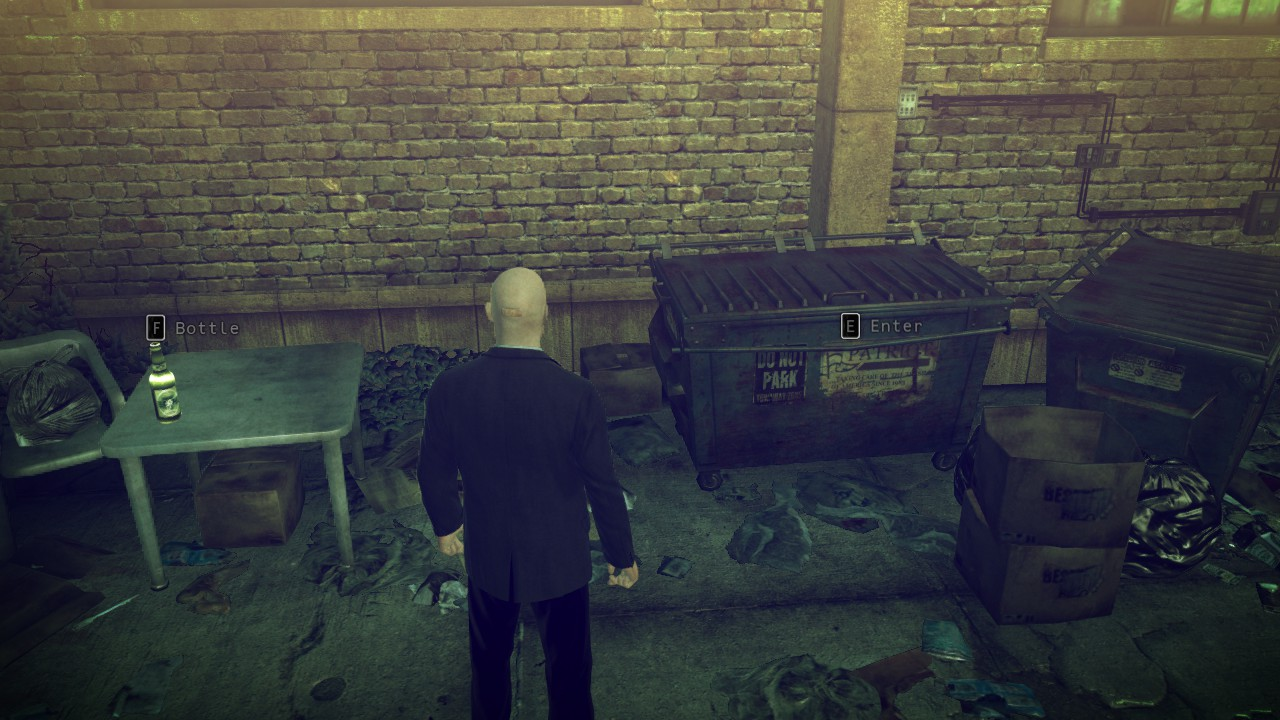
\includegraphics[width=11.5cm,keepaspectratio]{pics/shadows/ambientOcclusion/hitman}
  \end{figure}
\end{frame}

\begin{frame}
  \frametitle{Druhy stínů - Ambient occlusion}
  \begin{figure}[h]
    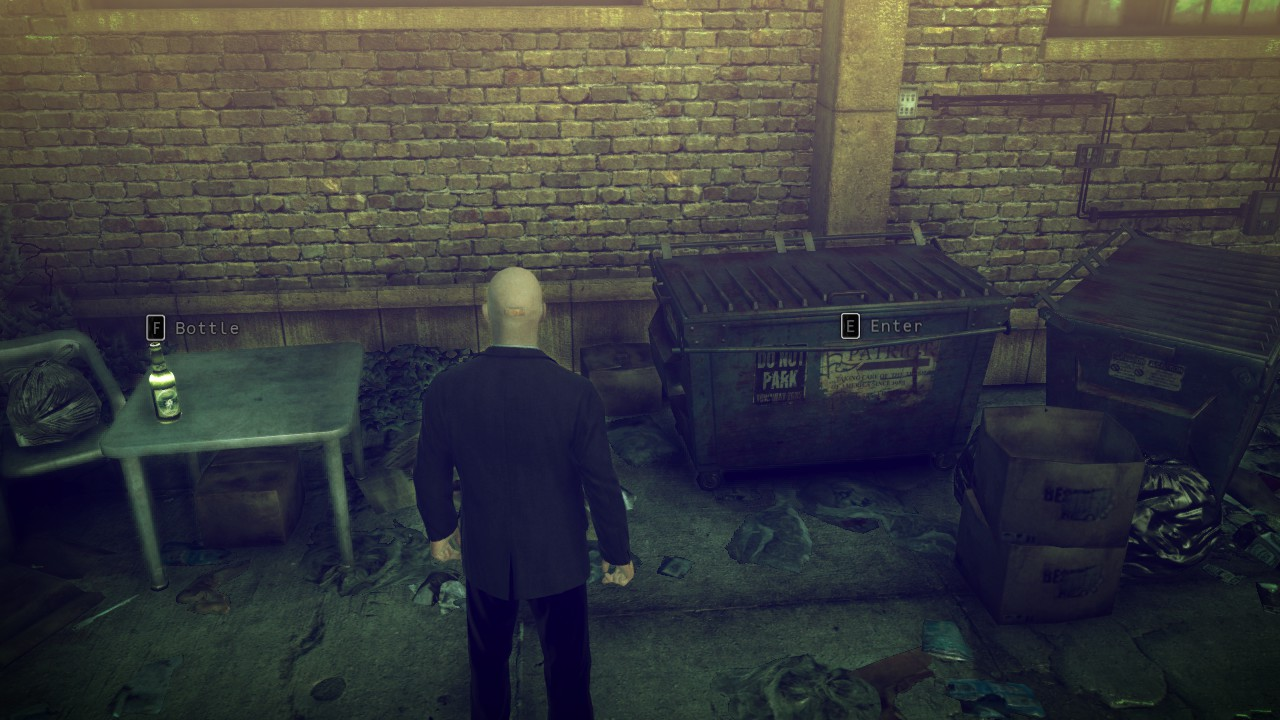
\includegraphics[width=11.5cm,keepaspectratio]{pics/shadows/ambientOcclusion/hitmanssao}
  \end{figure}
\end{frame}

\begin{frame}
  \frametitle{Druhy stínů - Ambient occlusion}
  \begin{figure}[h]
    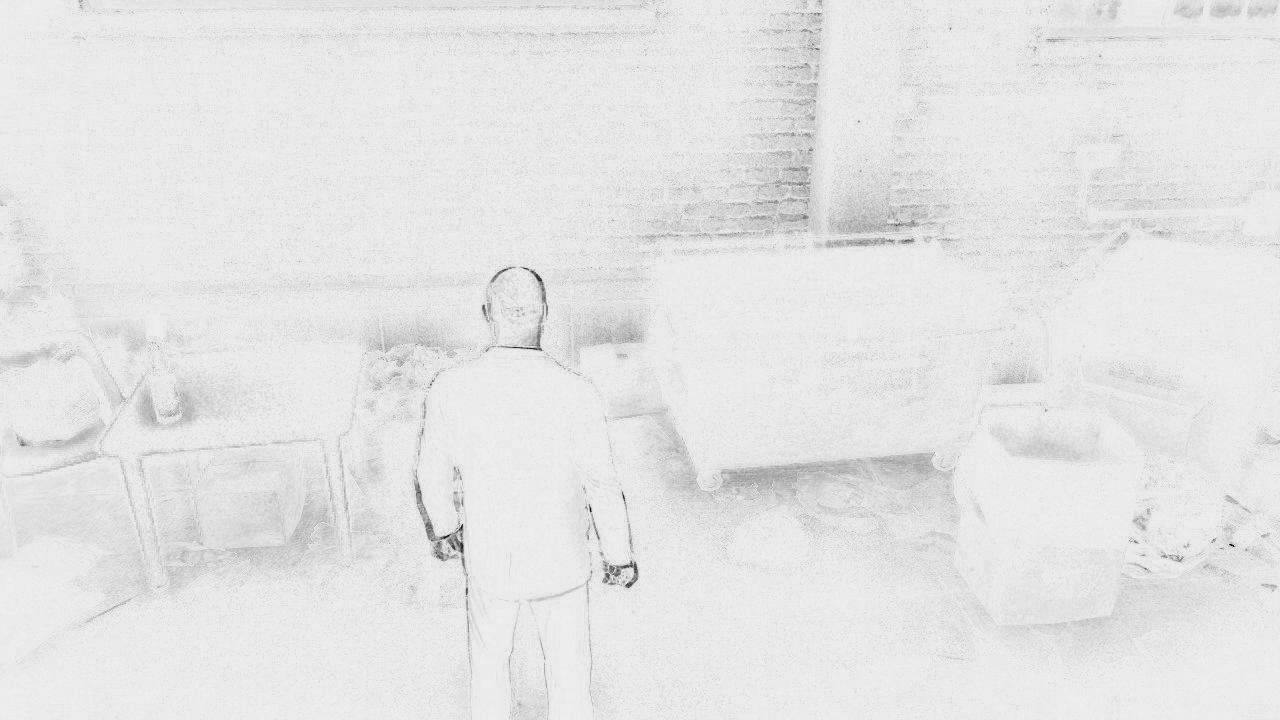
\includegraphics[width=11.5cm,keepaspectratio]{pics/shadows/ambientOcclusion/hitmanDifference}
  \end{figure}
\end{frame}
